\documentclass[12pt]{article}

\input{/home/iasbeck/preamble.tex}

\renewcommand{\headrulewidth}{0.5pt} % Redefine a espessura da lina no cabeçalho
\lhead{Modelagem e Otimização da estrutura do \textit{Ball and Plate}} % Lado esquerdo do cabeçalho
\chead{} % Centro do cabeçalho
\rhead{Arthur Iasbeck} % Lado direito  do cabeçalho
\lfoot{} % Lado esquerdo do rodapé
\cfoot{} % Centro do rodapé
\rfoot{\thepage} % Lado direito  do rodapé

% Folha A4
% Margem superior = Margem esquerda = 3cm
% Margem direita = Margem inferior = 2cm
% Fonte Times New Roman 12
% Títulos de Figuras e Tabelas Times New Roman 10
% Espaçamento simples e alinhamento justificado

% Início do documento
\begin{document}
	\singlespacing % Espaçamento simples
	
	\thispagestyle{empty}
	
	\begin{center}
		\huge
		Modelagem e Otimização da estrutura do \textit{Ball and Plate} \\~\\
	\end{center}
	
	O presente trabalho tem como objetivo a modelagem e otimização da estrutura do \textit{Ball and Plate} (BP), mais especificamente dos braços que conectam o motor à mesa. Um diagrama do sistema apresentando todas as grandezas consideradas é apresentado na Fig. \ref{diagramaBP}. 
	
	\begin{figure}[H]
		\centering
		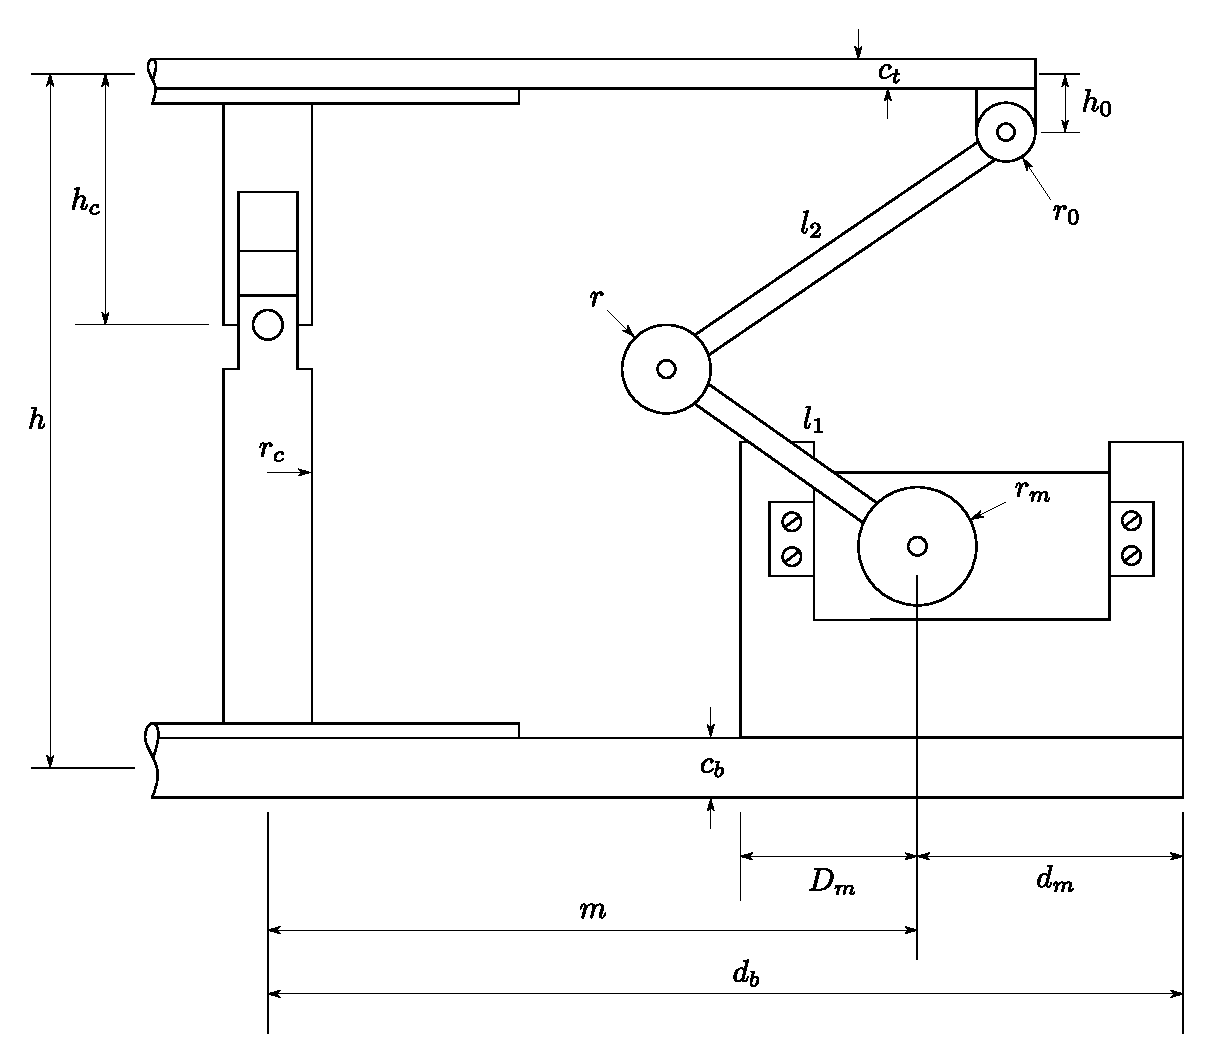
\includegraphics[width=1\linewidth]{figuras/diagramaBP.pdf}
		\caption{Vista lateral do sistema \textit{Ball and Plate}.}
		\label{diagramaBP}
	\end{figure}
	
	Quando o braço do motor se move, a estrutura parte de um estado inicial, em que a inclinação da mesa era nula, para um novo estado, ambos representados na Fig. \ref{diagramaSimples}.
	
	\begin{figure}[H]
		\centering
		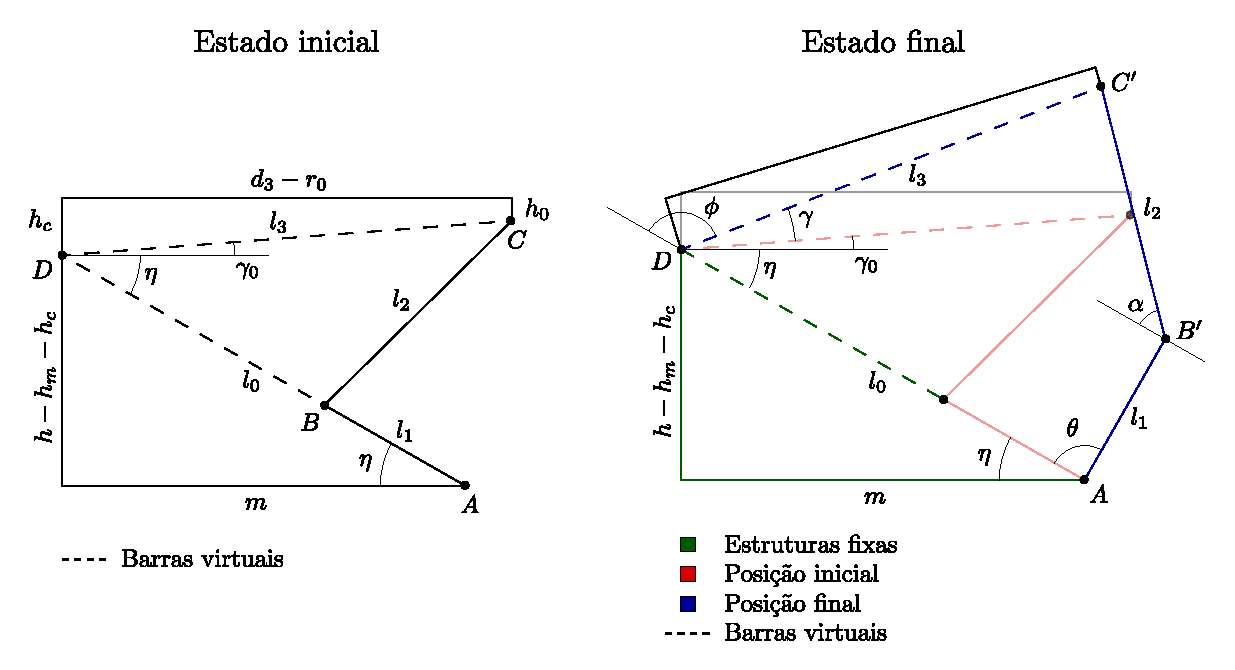
\includegraphics[width=1\linewidth]{figuras/diagramaSimples.pdf}
		\caption{Diagrama simplificado para análise do comportamento cinemático da estrutura.}
		\label{diagramaSimples}
	\end{figure}
	
	Avaliando a posição assumida pela estrutura no estado final, fica claro que os braços que conectam o motor à mesa formam um mecanismo de quatro barras, delimitado pelos pontos $ A $, $ B' $, $ C' $ e $ D $.
	
	Para modelar o mecanismo de quatro barras, Fig. \ref{4link}, é necessário primeiramente definir relações geométricas entre $ l_0 $, $ l_1 $, $ l_2 $ e $ l_3 $. Para tanto, basta avaliar as projeções de cada uma das barras tanto na horizontal, Eq. \ref{horizontal}, quanto na vertical, Eq. \ref{vertical}.
	\begin{figure}[H]
		\centering
		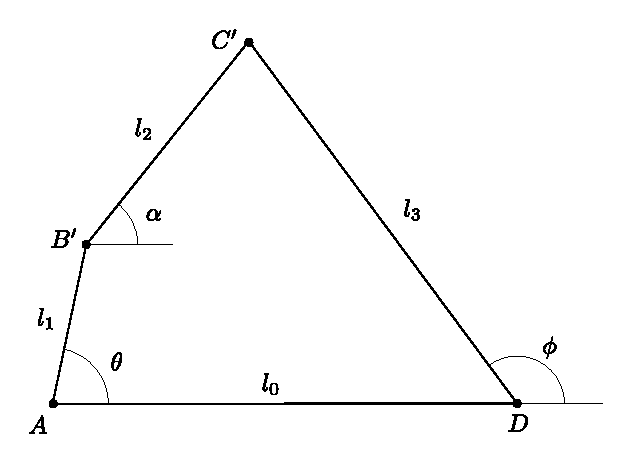
\includegraphics[width=0.6\linewidth]{figuras/4link.pdf}
		\caption{Diagrama simplificado do mecanismo de quatro barras composto pelos braços da estrutura do \textit{Ball and Plate}.}
		\label{4link}
	\end{figure}
	\begin{equation}
		\label{horizontal}
		\begin{gathered}
			l_0 - l_1 cos \theta - l_2 cos \alpha - l_3 cos(180 - \phi) = 0 \Rightarrow \\
			l_0 - l_1 cos \theta - l_2 cos \alpha - l_3 cos \phi = 0 
		\end{gathered}
	\end{equation}
	\begin{equation}
		\label{vertical}
		\begin{gathered}
			l_3 sen(180 - \phi) - l_1 sen\theta - l_2 sen \alpha = 0 \Rightarrow \\
			l_3 sen \phi - l_1 sen\theta - l_2 sen \alpha = 0
		\end{gathered}
	\end{equation}

	Uma vez que deseja-se obter a inclinação da mesa a partir da posição angular do motor, é necessário estabelecer uma relação entre $ \theta $ e $ \phi $. Visando-se a obtenção de $ \phi = f(\theta) $, isolam-se os termos dependentes de $\alpha$ nas Eqs. \ref{horizontal} e \ref{vertical}.
	\begin{equation}
		\label{isolaAlfa}
		\begin{gathered}
			l_2 cos \alpha = l_0 + l_3 cos \phi - l_1 cos \theta \\
			l_2 sin \alpha = l_3 sen \phi - l_1 sen \theta
		\end{gathered}
	\end{equation}
	
	Em seguida, elevam-se ao quadrado as Eqs. \ref{isolaAlfa} para posteriormente somá-las. Considerando o desenvolvimento apresentado na Eq. \ref{quadGenerica},
	\begin{equation}
		\label{quadGenerica}
		\begin{aligned}
			(A + B - C)^2 &= (A + B - C)(A + B - C) \\
			&= A^2 + AB - AC + AB + B^2 - BC - AC - BC + C^2  \\
			&= A^2 + B^2 + C^2 + 2AB - 2BC - 2AC
		\end{aligned}
	\end{equation}
	
	\noindent e assumindo
	\begin{equation}
		\begin{gathered}
			A = l_0 \\
			B = l_3 cos \phi \\
			C = l_1 cos \theta
		\end{gathered}
	\end{equation}

	\noindent são obtidas as relações apresentadas nas Eqs. \ref{quadrado},
	\begin{equation}
		\label{quadrado}
		\begin{aligned}
			l_2^2 cos^2 \alpha &= l_0^2 + l_3^2 cos^2 \phi + l_1^2 cos^2 \theta + 2 l_0 l_3 cos \phi - 2 l_3 l_2 cos \phi cos \theta - 2 l_0 l_1 cos \theta \\
			l_2^2 sen^2 \alpha &= l_3^2 sen^2 \phi + l_1^2 sen^2 \theta - 2 l_3 l_1 sen \phi sen \theta
		\end{aligned}
	\end{equation}
	
	\noindent que quando somadas resultam na relação introduzida na Eq. \ref{somaQuad}.
	\begin{equation}
		\label{somaQuad}
		\begin{aligned}
			l_2^2 (cos^2 \alpha + sen^2 \alpha) = & \;l_0^2 + l_3^2 (cos^2 \phi + sen^2 \phi) + l_1^2 (cos^2 \theta + sen^2 \theta) + \\
			&+2 l_0 l_3 cos \phi - 2 l_0 l_1 cos \theta - 2 l_3 l_1 cos \phi cos \theta - 2 l_3 l_1 sen \phi sen \theta
		\end{aligned}
	\end{equation}

	Reescrevendo a Eq. \ref{somaQuad} em função dos termos dependentes de $ \phi $ e adotando, a título de simplificação, constantes $ k_1 $, $ k_2 $ e $ k_3 $, é obtida a relação apresentada na Eq. \ref{eqTrig}. 
	\begin{gather}
		sen \phi (-2 l_3 l_1 sen \theta) + cos \phi (2 l_0 l_3 - 2 l_3 l_1 cos \theta) + (l_0^2 + l_1^2 - l_2^2 + l_3^2 - 2 l_0 l_1 cos \theta) = 0 \Rightarrow \nonumber \\
		k_1 sen \phi + k_2 cos \phi + k_3 = 0 \label{eqTrig}
	\end{gather}
	
	Para obtenção da solução da Eq. \ref{eqTrig}, adota-se uma variável auxiliar $ t $, definida da seguinte forma
	\begin{equation}
		t = tan \frac{\phi}{2} = \sqrt{\frac{1 - cos \phi}{1 + cos \phi}}
	\end{equation}
	
	Uma vez definida a variável auxiliar $ t $, é possível definir a partir dela uma relação para o cálculo do $ cos \phi $, Eq. \ref{cos},
	\begin{gather}
		t^2 = \frac{1 - cos \phi}{1 + cos \phi} \Rightarrow \nonumber\\
		t^2 + t^2 cos \phi = 1 - cos \phi \Rightarrow \nonumber\\
		cos \phi (t^2 + 1) = 1 - t^2 \Rightarrow \nonumber\\
		cos \phi = \frac{1 - t^2}{1 + t^2} \label{cos}
	\end{gather}
	
	\noindent e uma para o cálculo do $ sen \phi $, Eq. \ref{sen},
	\begin{gather}
		sen^2 \phi + cos^2 \phi = 1 \Rightarrow \nonumber\\
		sen \phi = \sqrt{1 - cos^2 \phi} = \sqrt{1 - \frac{(1 - t^2)^2}{(1 + t^2)^2}} = \sqrt{1 - \frac{1 - 2t^2 + t^4}{1 + 2t^2 + t^4}}\Rightarrow \nonumber\\
		sen \phi = \sqrt{\frac{1 + 2t^2 + t^4 - 1 + 2 t^2 - t^4}{1 + 2t + t^2}} \Rightarrow \nonumber\\
		sen \phi = \sqrt{\frac{4t^2}{(1 + t^2)^2}} \Rightarrow \nonumber\\
		sen \phi = \frac{2t}{1 + t^2} \label{sen}
	\end{gather}

	Introduzindo as Eqs. \ref{sen} e \ref{cos} na Eq. \ref{eqTrig}, obtêm-se uma relação para o cálculo de $ t $, Eq. \ref{calculoT}.
	\begin{gather}
		k_1 sen \phi + k_2 cos \phi + k_3 = 0 \nonumber \Rightarrow \\
		\frac{k_1 (2t) + k_2 (1 - t^2) + k_3 (1 + t^2)}{1 + t^2} = 0 \nonumber \Rightarrow \\
		t^2 (k_3 - k_2) + t (2 k_1) + (k_2 + k_3) = 0 \nonumber \Rightarrow \\
		t = \frac{-2 k_1 \pm \sqrt{4k_1^2 - 4(k_3 - k_2)(k_3 + k_2)}}{2 (k_3 - k_2)} \nonumber \Rightarrow \\
		t = \frac{-k_1 \pm \sqrt{k_1^2 + k_2^2 - k_3^2}}{k_3 - k_2} \label{calculoT}
	\end{gather}

	Uma vez que $ t = \frac{\phi}{2} $ por definição, segue que
	\begin{equation}
		\label{thetaPhi}
		\phi = 2 tan^{-1} \left( \frac{-k_1 \pm \sqrt{k_1^2 + k_2^2 - k_3^2}}{k_3 - k_2} \right)
	\end{equation}

	Uma vez que $ k_1 $, $ k_2 $ e $ k_3 $ dependem apenas dos comprimentos $ l_0 $, $ l_1 $, $ l_2 $ e $ l_3 $, e do ângulo $ \theta $, a Eq. \ref{thetaPhi} possibilita a relação entre a posição do motor, diretamente ligada a $ \theta $, e a inclinação da mesa, que depende de $ \phi $. 
	
	Uma vez determinado um modelo para o mecanismo de quatro barras, é necessário encontrar tanto a relação entre o ângulo $ \theta $ e a posição angular do motor $ \theta_m $, quanto aquela entre o ângulo $ \phi $ e a inclinação da mesa $ \phi $. Estas relações, e algumas outras, introduzidas nas Eqs. \ref{relacoesBP}, podem ser obtidas pela análise do diagrama apresentados na Fig. \ref{diagramaSimples} e serão de suma importância na determinação dos comprimentos dos braços da estruturas (representados por $ l_1 $ e $ l_2 $). Cabe ressaltar que adotou-se que as barras $ l_0 $ e $ l_1 $ estarão alinhadas quando a mesa estiver alinhada com a horizontal (caso em que $ \gamma = \theta = 0 $). Desta forma, $ \theta = \theta_m $ e é possível obter o comprimento $l_2$ por meio da análise do triângulo $ BCD $, Fig. \ref{diagramaSimples}.
	\begin{equation}
		\label{relacoesBP}
		\begin{gathered}
			\theta = \theta_m \\
			\eta = tan\left( \frac{h - h_m - h_c}{m} \right) \\
			\gamma_0 = tan^{-1} \left( \frac{h_c - h_0}{d_3 - r_0} \right) \\
			\phi = 180 - \eta - \gamma_0 - \phi \\
			l_0 = \sqrt{m^2 + (h - h_m h_c)^2} \\
			l_3 = \sqrt{(h_c - h_0)^2 + (d_3 - r_0)^2} \\
			l_2 = \sqrt{(l_0 - l_1)^2 + l_3^2 - 2 l_3 (l_0 - l_1) cos (\eta + \gamma_0)}
		\end{gathered}
	\end{equation}

	Pela avaliação das Eqs. \ref{relacoesBP} conclui-se que para determinar as dimensões dos braços do BP é necessário que sejam determinados a posição $ m $ do motor com relação ao centro da mesa, e o comprimento $ l_1 $ do braço diretamente conectado ao motor. 

	Visando a simplificação do modelo dinâmico do BP, pretende-se escolher $ l_1 $ e $ m $ de forma que $ \gamma \approx \theta $, como indica a Fig. \ref{respostaOtm}. Para tanto, é necessário que a diferença entre as curvas, representada por $ e $ seja a menor possível. Assim sendo, pode-se determinar $ l_1 $ e $ m $ minimizando $ J $, Eq. \ref{fobj}.
	\begin{equation}
		\label{fobj}
		J = \int_{-30^o}^{30^o} e(l_1, m)^2 d\theta
	\end{equation} 

	Foram escolhidos como limites de integração $ \theta = -30^o $ e $ \theta = 30^o $ para que fosse possível adotar na modelagem dinâmica do BP as simplificações $ sen \theta = \theta $ e $ sen \gamma = \gamma $. 
	\begin{figure}[H]
		\centering
		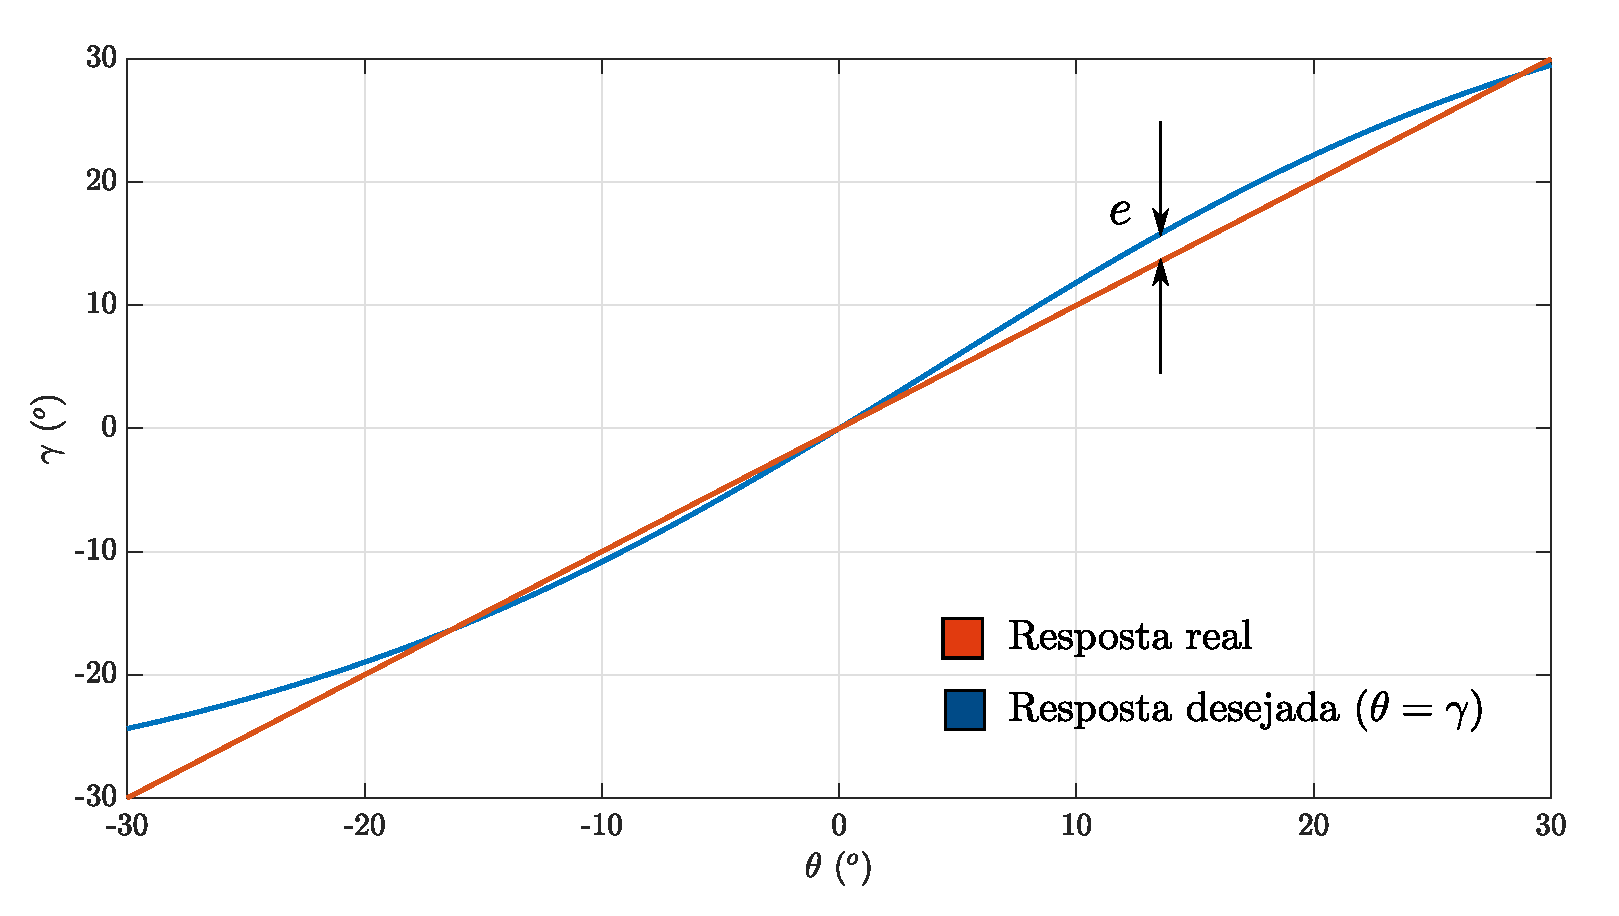
\includegraphics[width=\linewidth]{figuras/respostaOtm.pdf}
		\caption{Comparação entre a relação real entre $ \theta $ e $ \gamma $ e a relação que deseja-se obter a partir do processo de otimização, em que $ \theta = \gamma $.}
		\label{respostaOtm}
	\end{figure}

	Uma vez estabelecida a função a ser minimizada, é necessário estabelecer os limites laterais para $ m $ e $ l_1 $. Estas podem ser obtidas da análise do diagrama introduzido na Fig. \ref{diagramaBP}. Os limites para $ m $ são apresentados na Eq. \ref{limM}.
 	\begin{equation}
 		\label{limM}
	 	r_c + D \leq m \leq d_b - d_m \\
 	\end{equation}
 	
 	Como valor máximo para $ l_1 $ adotou-se o próprio $ l_0 $, uma vez que considerou-se que $ l_0 $ e $ l_1 $ estão alinhados quando $ \gamma = 0 $. Uma vez que $ l_0 $ depende de $ m $, o valor máximo de $ l_1 $ também dependerá. Foi assumido neste caso o valor máximo de $ m $, uma vez que trata-se de um limite superior para $ l_1 $.
 	\begin{gather}
 		0 \leq l_1 \leq l_0 \Rightarrow \nonumber\\
 		0 \leq l_1 \leq \sqrt{m^2 + (h - h_m)^2} \Rightarrow \nonumber\\
 		0 \leq l_1 \leq \sqrt{(d_b - d_m)^2 + (h - h_m)^2} 
 	\end{gather}
 	
 	Além disso, é necessário estabelecer algumas restrições geométricas que empeçam que o braço do motor se choque com quaisquer outras partes da estrutura. Para impedir que o mesmo se choque com o suporte da mesa, adotou-se a restrição introduzida na Eq. \ref{rest1}, deduzida a partir da análise do diagrama introduzido na Fig. \ref{diagramaBP}.
	\begin{equation}
		\label{rest1}
		\begin{gathered}
			l_1 + r \leq m - r_c \Rightarrow \\
			l_1 + r - m + r_c \leq 0
		\end{gathered}
	\end{equation}
	
	Uma vez que o aumento do braço do motor acarreta a diminuição de $ J $, como foi possível comprovar por meio de experimentações numéricas, a execução do processo de otimização acaba por ativar sempre esta restrição. Para evitar problemas com a montagem do sistema, adotou-se a adição de $ 1 \;\; cm $ na restrição estabelecida inicialmente. 
	\begin{equation}
		l_1 + r - m + r_c + 0,01 \leq 0
	\end{equation}
	
	Além disso, é necessário que o braço do motor não se choque com a base do BP. Para impedir que isto ocorra, outra restrição, Eq. \ref{eq:rest2} foi levada em consideração. Sua dedução advém da análise do diagrama apresentado na Fig. \ref{rest2} e na consideração de que o $ -30^o \leq \theta \leq 30^o $. 
	\begin{gather}
	\label{eq:rest2}
	h_r + r \leq h_m - \frac{c_b}{2} \nonumber \Rightarrow \\
	l_1 sen(\eta - 30^o) + r - h_m + \frac{c_b}{2} \leq 0
	\end{gather}
	
	\begin{figure}[H]
		\centering
		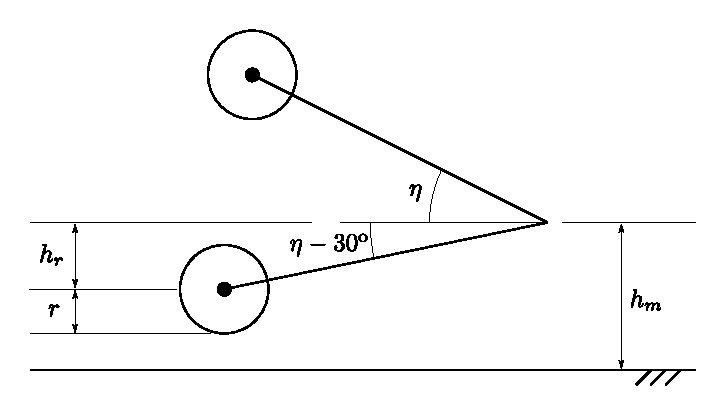
\includegraphics[width=0.7\linewidth]{figuras/rest2.pdf}
		\caption{Diagrama simplificado do braço do motor em sua posição limite.}
		\label{rest2}
	\end{figure}
	
	Considerando o que foi apresentado até o momento, as relações que resumem o processo de otimização a ser implementado são resumidas nas Eqs. \ref{otmFinal}.
	\begin{equation}
		\label{otmFinal}
		\begin{gathered}
			\underset{m, l_1 \, \in \; {\rm I\!R}}{min} \; J = \int_{-30^o}^{30^o} e \, d\theta \\
			l_1 + r - m + r_c + 0,01 \leq 0 \\
			l_1 sen(\eta - 30^o) + r - h_m + \frac{c_b}{2} \leq 0 \\
			r_c + D \leq m \leq d_b - d_m \\
			0 \leq l_1 \leq \sqrt{(d_b - d_m)^2 + (h - h_m)^2} \\
		\end{gathered}
	\end{equation}
	
	Por meio de medições realizadas no sistema já construído foram obtidas para as grandezas introduzidas no diagrama apresentado na Fig. \ref{diagramaBP} os valores numéricos exibidos na Tab. \ref{tabGrand}. Os códigos utilizados para obtenção da solução do problema de otimização proposto são apresentados em seguida. É importante ressaltar que o problema foi resolvido utilizando-se palpites iniciais igualmente distribuídos pelo espaço de busca, uma vez que a determinação destes pode afetar a solução do problema. 
	
	\begin{table}[H]
		\centering
		\caption{Valores das grandezas introduzidas no diagrama apresentado na Fig. \ref{diagramaBP} em metros.}
		\label{tabGrand}
		\begin{tabular}{|c|c|c|c|c|c|}
			\hline
			$h_c$ & 0,0540 & $h_0$ & 0,0300 & $d_m$ & 0,0290 \\ \hline
			$d_3$ & 0,1500 & $r$   & 0,0100 & $D_m$ & 0,0510 \\ \hline
			$h$   & 0,1625 & $r_0$ & 0,0120 & $r_c$ & 0,0130 \\ \hline
			$h_m$ & 0,0425 & $d_b$ & 0,2000 & $c_b$ & 0,0150 \\ \hline
		\end{tabular}
	\end{table}

\begin{lstlisting}
% main.m
	
clc; clear; close all;

% Inicializacao de variaveis
results = zeros(100,3);
k = 1;
% Funcao objetivo e restricoes
f = @fObj;
c = @const;
% Restricoes de desigualdade
A = [];
b = [];
% Restricoes de igualdade
Aeq = [];
beq = [];
% Limites laterais
h = 0.1625;
hc = 0.084;
hm = 0.0425;
db = 0.2;
dm = 0.029;
Dm = 0.051;
rc = 0.013;

lb = [0, rc+Dm];
ub = [sqrt((db-dm)^2+(h-hm-hc)^2), db-dm];

for x01 = linspace(0,0.1,10)
	for x02 = linspace(0,0.15,10)
		% Palpite inicial
		x0 = [x01, x02];
		% Processo de otimizacao
		[x, fval] = fmincon(f,x0,A,b,Aeq,beq,lb,ub,c);
		results(k, 1:2) = x;
		results(k, 3) = fval;
		k = k + 1;
	end
end

disp('Fim da execucao');
\end{lstlisting}

\begin{lstlisting}
% fObj.m

function f = fObj(x)

l1 = x(1); % Braco do motor
m = x(2); % Distancia do motor ate o centro da mesa

nData = 100;
hc = 0.054;
d3 = 0.15;
h = 0.1625;
hm = 0.0425;
h0 = 0.03;
r0 = 0.012;

l3 = sqrt((hc-h0)^2 + (d3-r0)^2);
thetaMValues = linspace(-pi/6,pi/6,nData); % Angulos que o motor assume
gamaValues = zeros(nData,1); % Vetor que guarda os valores de inclinacao da mesa

n = atan((h-hm-hc)/m); % Angulo entre l0 e a horizontal
gama0 = atan((hc-h0)/(d3-r0));
l0 = sqrt((h-hm-hc)^2 + m^2);
l2 = sqrt((l0 - l1)^2 + l3^2 - 2*l3*(l0-l1)*cos(n+gama0));

for j = 1:nData
	thetaM = thetaMValues(j);
	theta = thetaM;
	k1 = -2*l1*l3*sin(theta);
	k2 = 2*l3*(l0 - l1*cos(theta));
	k3 = l0^2 + l1^2 - l2^2 + l3^2 - 2*l0*l1*cos(theta);
	phi = 2*atan((-k1 - sqrt(k1^2 + k2^2 - k3^2))/(k3 - k2));
	gama = pi - n - gama0 - phi;
	gamaValues(j) = gama;
end

linGama = linspace(-pi/6,pi/6,nData)'; % Reta de 45 graus que relaciona theta e gamma

e = (gamaValues - linGama).^2; % Diferenca entre a aproximacao linear e os valores reais
dTheta = thetaMValues(2) - thetaMValues(1); % Calculo do incremento de theta
ie = sum(e*dTheta); % Calculo da integral do erro
f = ie; % Valor da funcao objetivo
\end{lstlisting}

\begin{lstlisting}
% const.m

function [c, ceq] = const(x)

rc = 0.013;
r = 0.01;
h = 0.1625;
hm = 0.0425;
hc = 0.054;
cb = 0.015;

l1 = x(1); % Braco do motor
m = x(2); % Distancia do motor ate o centro da mesa

n = atan((h-hm-hc)/m); % Angulo entre l0 e a horizontal

c = [l1 + r - m + rc
l1*sin(n - pi/6) + r - hm + cb/2];
ceq = [];
\end{lstlisting}

\begin{lstlisting}
clc; clear; close all;

x = [0.096436 0.17099]; 

c = const(x);

fprintf('Restricao 1 = %f cm \n', c(1)*100);
fprintf('Restricao 2 = %f cm \n', c(2)*100);

l1 = x(1); % Braco do motor
m = x(2); % Distancia do motor ate o centro da mesa

nData = 100;
hc = 0.054;
d3 = 0.15;
h = 0.1625;
hm = 0.0425;
h0 = 0.03;
r0 = 0.012;

l3 = sqrt((hc-h0)^2 + (d3-r0)^2);
thetaMValues = linspace(-pi/6,pi/6,nData); % Angulos que o motor assume
gamaValues = zeros(nData,1); % Vetor que guarda os valores de inclinacao da mesa

n = atan((h-hm-hc)/m); % Angulo entre l0 e a horizontal
gama0 = atan((hc-h0)/(d3-r0));
l0 = sqrt((h-hm-hc)^2 + m^2);
l2 = sqrt((l0 - l1)^2 + l3^2 - 2*l3*(l0-l1)*cos(n+gama0));

for j = 1:nData
	thetaM = thetaMValues(j);
	theta = thetaM;
	k1 = -2*l1*l3*sin(theta);
	k2 = 2*l3*(l0 - l1*cos(theta));
	k3 = l0^2 + l1^2 - l2^2 + l3^2 - 2*l0*l1*cos(theta);
	phi = 2*atan((-k1 - sqrt(k1^2 + k2^2 - k3^2))/(k3 - k2));
	gama = pi - n - gama0 - phi;
	gamaValues(j) = gama;
end

linGama = linspace(-pi/6,pi/6,nData)'; % Reta de 45 graus que relaciona theta e gamma

e = (gamaValues - linGama).^2; % Diferenca entre a aproximacao linear e os valores reais
dTheta = thetaMValues(2) - thetaMValues(1); % Calculo do incremento de theta
ie = sum(e*dTheta); % Calculo da integral do erro
f = ie; % Valor da funcao objetivo

% Apresentacao grafica dos resultados
figure;
plotI(thetaMValues*180/pi, gamaValues*180/pi, '-'); hold on;
plotI(thetaMValues*180/pi, linGama*180/pi, '-');
xlabelI('$\theta$ ($^o$)');
ylabelI('$\gamma$ ($^o$)');
cropPlotI;
printI('bracoOtimizado');

% Relatorio
fprintf('Braco do motor = %.2f cm \n', l1*100);
fprintf('Braco auxiliar = %.2f cm \n', l2*100);
fprintf('Posicao do motor = %.2f cm \n', m*100);
fprintf('Angulo entre a posicao inicial do braco do motor e a horizontal = %.2f graus \n', n*180/pi);
fprintf('Valor da funcao objetivo = %f \n', f);

relErr = abs(gamaValues - linGama)./linGama;
eAbs = abs(gamaValues - linGama);

fprintf('Erro relativo maximo entre as curvas = %.2f %% (%.2f graus)\n', 100*max(abs(relErr)), 180/pi*max(eAbs));

B = gamaValues; % Dado real
f = linGama; % Dado ajustado
Bbar = mean(B);
SStot = sum((B - Bbar).^2);
SSres = sum((B - f).^2);
R2 = 1 - SSres/SStot;

fprintf('Correlacao entre as curvas (R2) = %.2f %% \n', R2*100);
\end{lstlisting}

	\vspace{0.4cm}
	Os resultados obtidos a partir da execução dos códigos introduzidos acima são apresentados a seguir.
	
\begin{lstlisting}
Restricao 1 (centro da mesa) = -5.155400 cm 
Restricao 2 (base da mesa) = -3.990973 cm 
Braco do motor (l1) = 9.64 cm 
Braco auxiliar (l2) = 7.94 cm 
Posicao do motor (m) = 17.10 cm 
Angulo entre l_1 (posicao inicial) e a horizontal = 21.11 graus
Valor da funcao objetivo (J) = 0.002085 
Erro relativo maximo entre as curvas (porcentagem) = 25.63 (7.69 graus)
Correlacao entre as curvas (R2) (porcentagem) = 97.65 
\end{lstlisting}
	
	\begin{figure}[H]
		\centering
		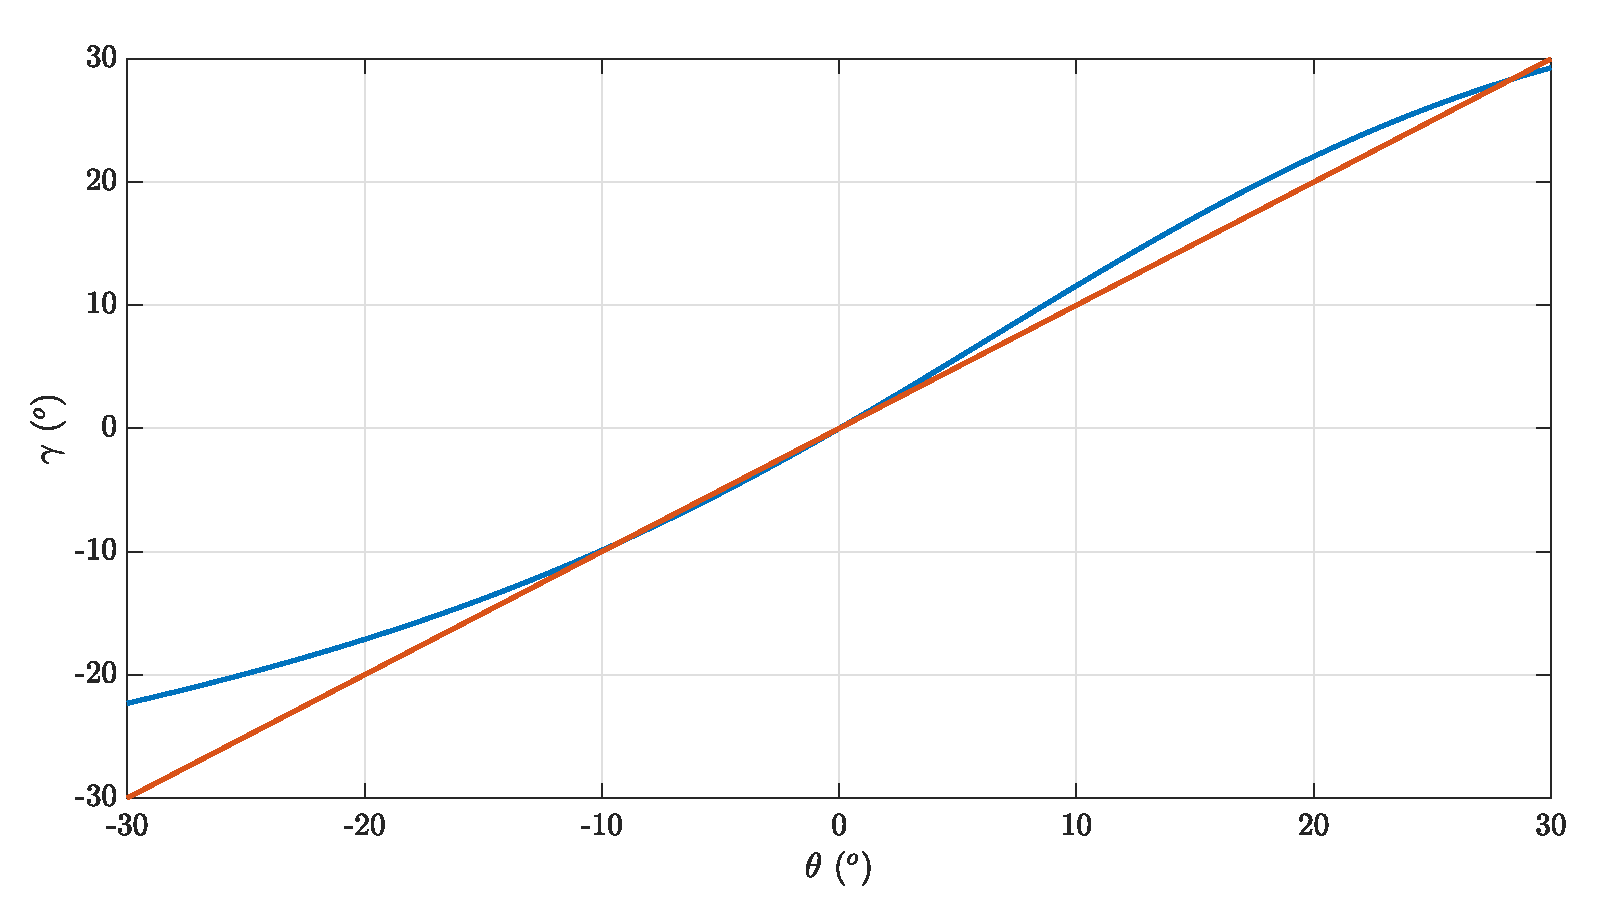
\includegraphics[width=\linewidth]{figuras/bracoOtimizado.pdf}
		\caption{Relação entre $ \theta $ e $ \gamma $ considerando $ l_1 $ e $ m $ obtidos após o processo de otimização}
		\label{bracoOtimizado}
	\end{figure}

\end{document}